\documentclass[12pt]{article}

%%%%%%%%%%%%%%%%%%%%%%%%%%%%
%%%%%%%%%%%%%%%%%%%%%%%%%%%%
% Load in packages
\usepackage{amsmath}
\usepackage{float}
\usepackage{amssymb}
\usepackage{hyperref}
\usepackage{graphicx}
\usepackage[top=1in, bottom=1in, left=1in, right=1in]{geometry}

%%%%%%%%%%%%%%%%%%%%%%%%%%%%
%%%%%%%%%%%%%%%%%%%%%%%%%%%%

\begin{document}

\begin{center}
\Large Chapter 6 Practice Problems

\medskip

\normalsize Elements of Microeconomics (discussion section 4)

\medskip

\small Jamie Hyder
\end{center}

\section*{Question 1}
This question will consider a market for coffee, which is depicted in figure \ref{fig:coffee_eq}.

\begin{figure}[h]
    \centering
    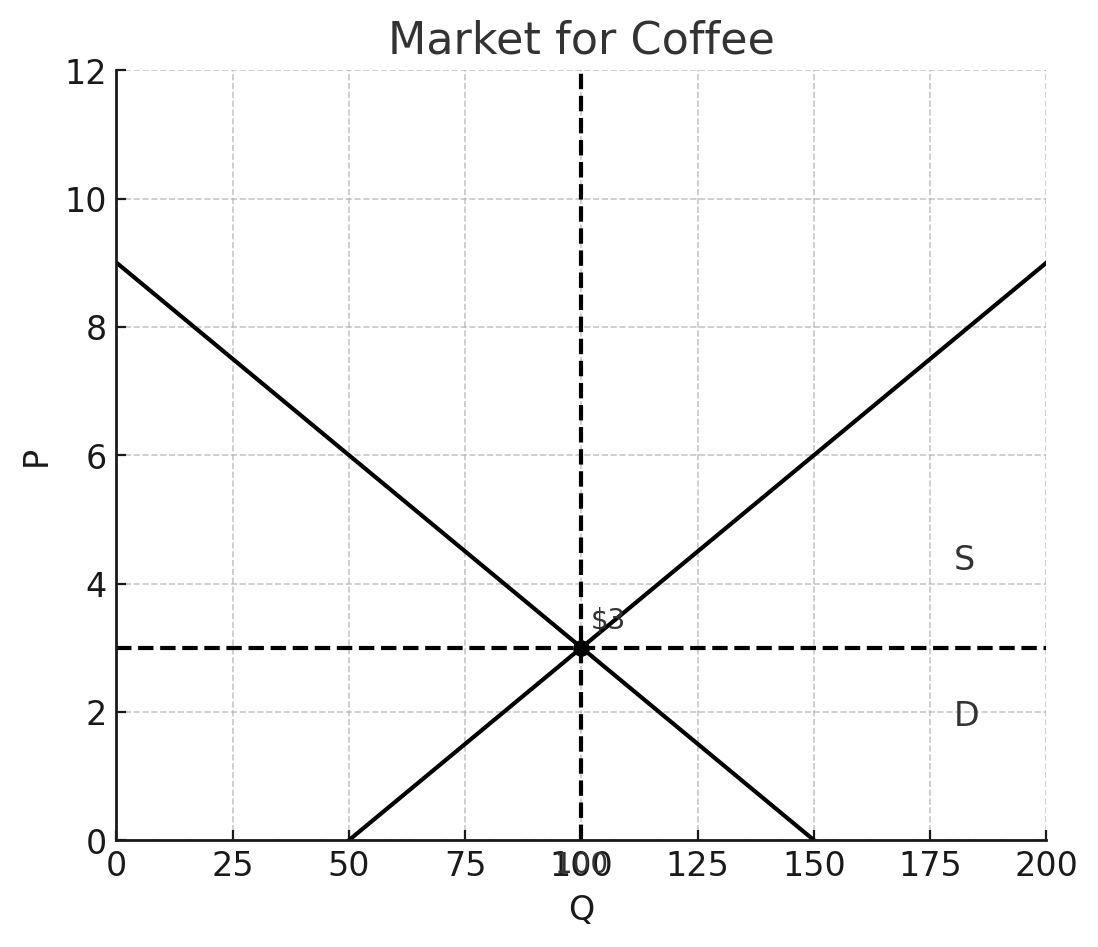
\includegraphics[width=.6\textwidth]{output-2.png}
    \caption{Market for coffee}
    \label{fig:coffee_eq}
\end{figure}

\begin{enumerate}

\item Consider two price ceilings:
    \begin{itemize}
        \item At \$2.5
        \item At \$3.5
    \end{itemize}

    \vspace{5mm}

    In both of these cases depict graphically the new market outcome, and answer:
    \begin{enumerate}
        \item What happens to the new quantity demanded and supplied?
        \item Does the policy cause a shortage or a surplus?
        \item Is the policy binding? Why or why not?
    \end{enumerate}

    \textbf{Answer:}
The policies are depicted in figures \ref{fig:coffee_ceiling_250} and \ref{fig:coffee_ceiling_350}.

\begin{figure}
    \centering
    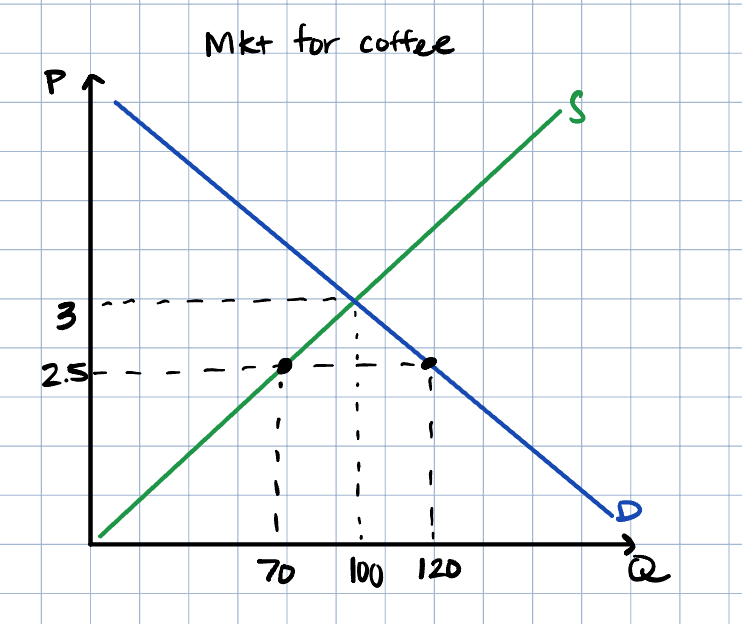
\includegraphics[width=.6\textwidth]{coffee_ceiling_250.png}
    \caption{Price ceiling at \$2.5}
    \label{fig:coffee_ceiling_250}
\end{figure}

\begin{figure}
    \centering
    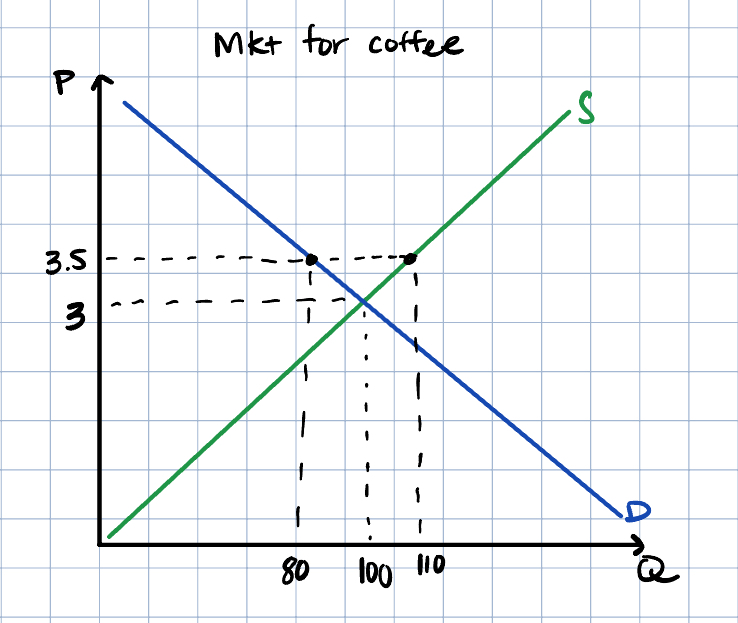
\includegraphics[width=.6\textwidth]{coffee_ceiling_350.png}
    \caption{Price ceiling at \$3.5}
    \label{fig:coffee_ceiling_350}
\end{figure}


\vspace{2mm}

You do not have enough information to determine the new levels of price and supply, but you can tell in what direction (if any) they move. The price ceiling at \$2.5 is binding because it is below the previous equilibrium price. Since price has gone down, demand must increase, and supply must decrease. This creates a shortage, where more consumers would like to \textit{buy} coffee at \$2.5 per cup than suppliers would like to \textit{sell} coffee at that price. This is the definition of a \textit{shortage}.

\vspace{2mm}

In contrast, the price ceiling at \$3.5 is not binding because it was above the equilibrium. No suppliers were selling above \$3 before, and so no one is effected by the ceiling.



\item Repeat the same exercise but for a price \textit{floor} at \$2.5 and \$3.5.

\textbf{Answer:}
The policies are depicted in figures \ref{fig:coffee_floor_250} and \ref{fig:coffee_floor_350}. They look the saame as those for the price ceiling, though they take on new meaning here...

\begin{figure}
    \centering
    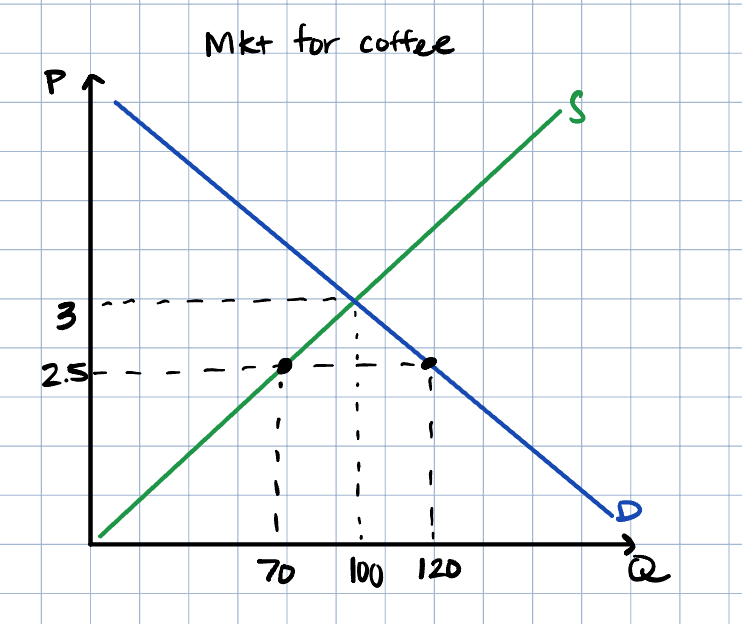
\includegraphics[width=.6\textwidth]{coffee_ceiling_250.png}
    \caption{Price floor at \$2.5}
    \label{fig:coffee_floor_250}
\end{figure}

\begin{figure}
    \centering
    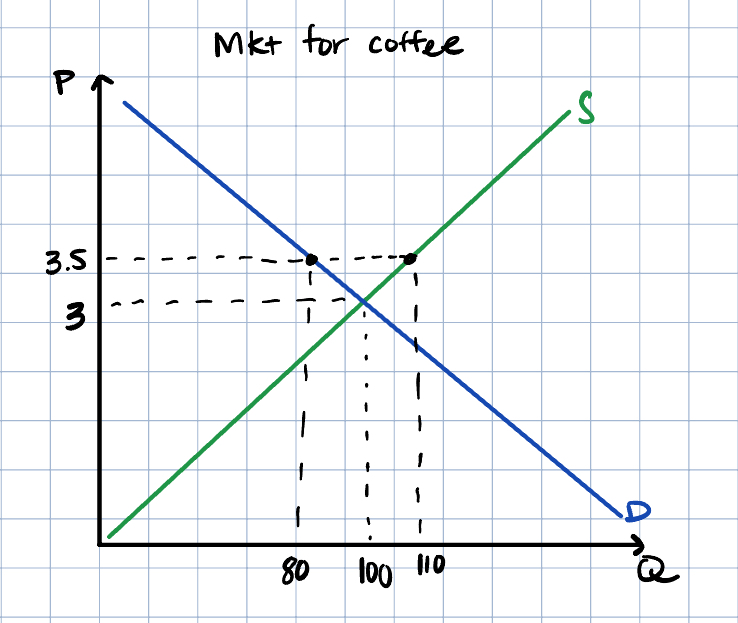
\includegraphics[width=.6\textwidth]{coffee_ceiling_350.png}
    \caption{Price floor at \$3.5}
    \label{fig:coffee_floor_350}
\end{figure}

\vspace{2mm}

The price floor at \$2.5 will not be binding, since this is lower than the equilibrium price. There are thus no changes to price or quantity, and no shortage or surplus.

\vspace{2mm}

However, the price floor at \$3.5 will bind. It will create a surplus, because at this high of a price, more suppliers would like to \textit{sell} their coffee than consumers would like to \textit{buy} it.

\end{enumerate}

\section*{Question 2}

\begin{enumerate}
\item Consider the market for Orioles tickets:
\begin{enumerate}
    \item Which side is elastic?
    \item Which side is inelastic?
    \item What might happen in the long run?
\end{enumerate}

Draw two graphs illustrating your answers, one in the short-run and one in the long-run.

\textbf{Answer:}
As we said before, supply for Orioles tickets is (nearly) perfectly inelastic in the short-run, since the owners of the team cannot increase or decrease the number of seats in Camden Yards. In the long-run, however, they may adjust buy building a new stadium; however this is incredibly costly, and so the long-run supply curve will likely also be inelastic (but more elastic than before).

\vspace{2mm}

We would expect demand in the short-run to be relatively elastic, since going to a sporting event is a luxury that most families can do without. There are also some fairly close substitutes, such as going to see the Ravens or a DC sports team. We would not expect the elasticity to change too much in the short- vs long-run; although consumers might switch teams or choose to get into a different sport, our taste in sports and in teams is largely determined by our families and experiences when we are young. 

\vspace{2mm}

Figures \ref{fig:Orioles_short} and \ref{fig:Orioles_long} depict the short- and long-run scenarios we described above: perfectly inelastic supply becomes slightly more elastic, and elastic demand remains relatively similar.

\begin{figure}
    \centering
    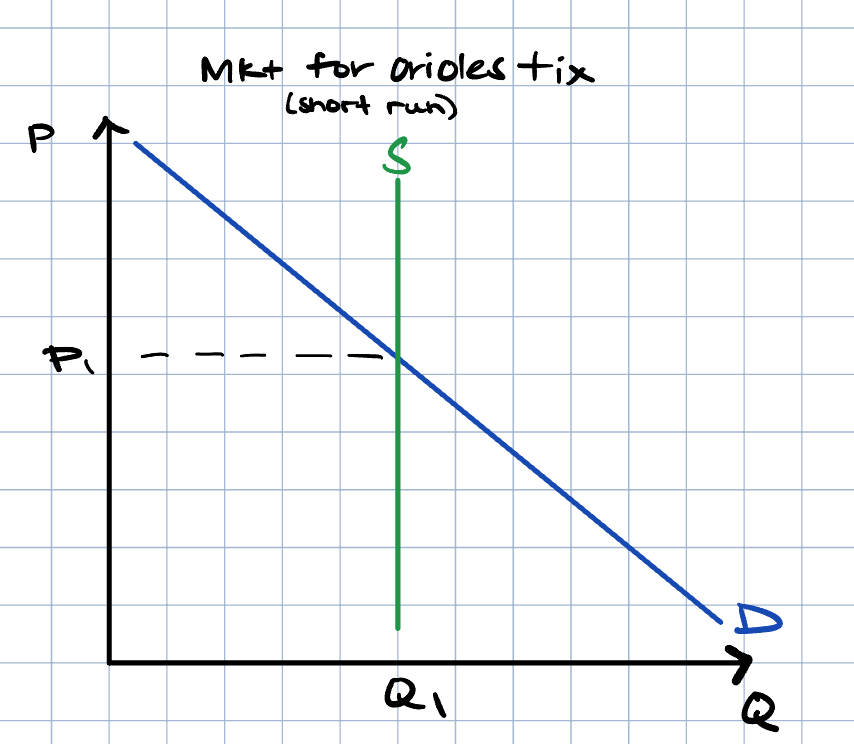
\includegraphics[width=.6\textwidth]{Orioles_short.png}
    \caption{Short-run market for Orioles tickets}
    \label{fig:Orioles_short}
\end{figure}

\begin{figure}
    \centering
    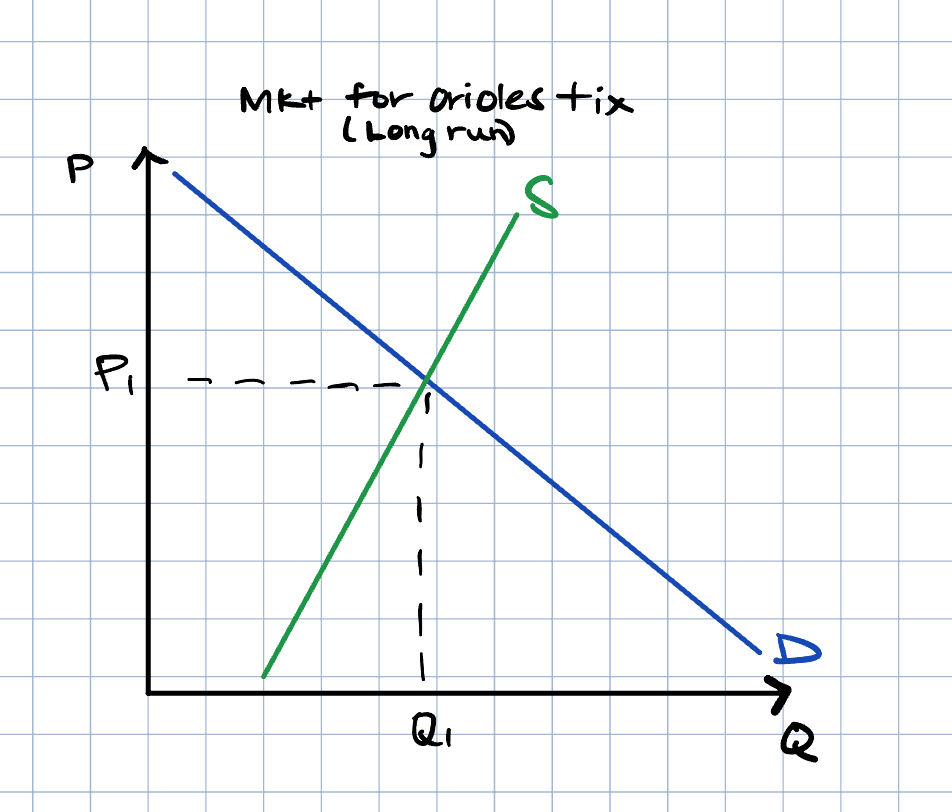
\includegraphics[width=.6\textwidth]{Orioles_long.png}
    \caption{Long-run market for Orioles tickets}
    \label{fig:Orioles_long}
\end{figure}

\item Now suppose Baltimore City imposes a \textit{binding} price floor on tickets:
    \begin{enumerate}
        \item What is the impact in the short-run?
        \item What is the impact in the long-run?
        \item Is the impact larger in the short-run or long-run?
    \end{enumerate}

    \textbf{Answer:}

Figures \ref{fig:Orioles_floor_short} and \ref{fig:Orioles_floor_long} depict the short- and long-run effects of a binding price floor. In both cases the price floor creates a surplus, because the Orioles owners would like to sell more tickets than consumers want to buy. However in the short-run the owners cannot increase their supply; in the long-run they can, which means that if the demand curve is relatively unchanged the surplus must be larger in the long-run than in the short run.


\begin{figure}
    \centering
    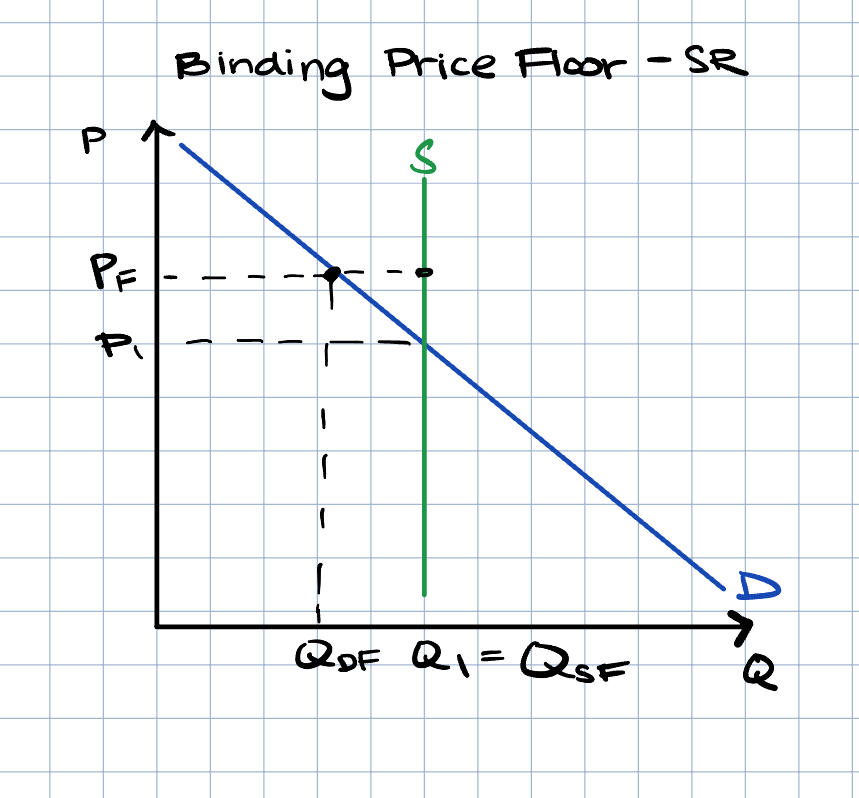
\includegraphics[width=.6\textwidth]{Orioles_floor_short.png}
    \caption{Short-run market with a price floor}
    \label{fig:Orioles_floor_short}
\end{figure}

\begin{figure}
    \centering
    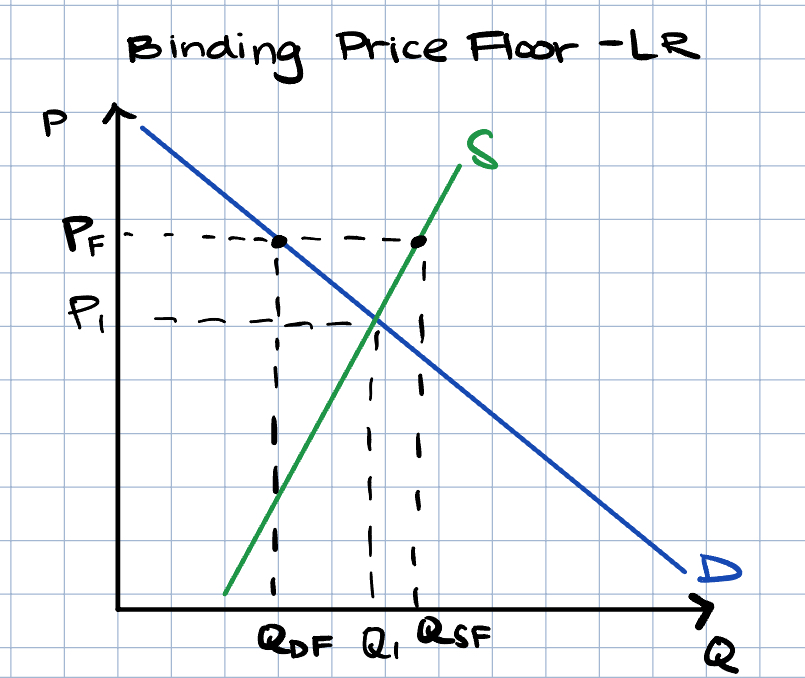
\includegraphics[width=.6\textwidth]{Orioles_floor_long.png}
    \caption{Long-run market with a price floor}
    \label{fig:Orioles_floor_long}
\end{figure}

\vspace{2mm}

Of course, what assumptions you make about the demand curve's long-run elasticity will impact your answer. If you thought that demand was inelastic in the long-run, it's possible that the shortage would be smaller.


    \end{enumerate}

\section*{Question 3}
\begin{enumerate}
\item Let's consider the coffee market from Question 1 again. Instead of price controls (rare in advanced economies), consider a tax of \$0.5 per cup applied to suppliers:

\begin{enumerate}
    \item Does this shift supply or demand curves?
    \item What will happen to equilibrium price and quantity?
    \item What portion falls on consumers and what falls on suppliers?
\end{enumerate}

 Draw a graph to illustrate the intuition behind your answers (I am not looking for specific numbers since you are not provided with functions). Make sure to draw the tax wedge, labeling the portion falling on consumers and on suppliers.

\vspace{2mm}
\textbf{Answer:}
Your depiction of the tax might look like figure \ref{fig:coffee_tax_1}.

\begin{figure}
    \centering
    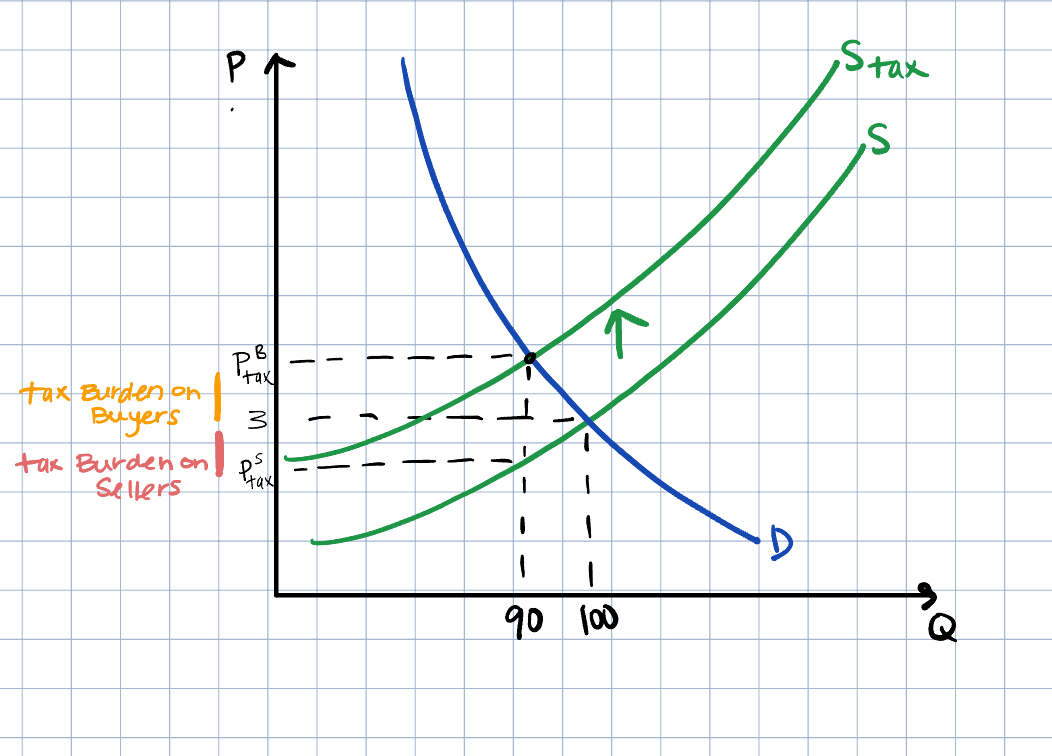
\includegraphics[width=.6\textwidth]{coffee_tax_1.png}
    \caption{Tax on coffee suppliers}
    \label{fig:coffee_tax_1}
\end{figure}

The tax is on suppliers, and so it shifts the supply curve and does not affect the demand curve (nothing fundamental about demand, eg tastes or the prices of substitutes, etc., was changed). At any given price, suppliers will supply less coffee than before, since they have to turn over \$0.5 to the government. This means that equilibrium price will increase and quantity will decrease.

\vspace{2mm}

The portion which falls on consumers and suppliers depends on the relative elasticities. In this depiction I drew an inelastic curve for consumers (who are very addicted to coffee, and are willing to pay a high price to fuel their addiction) and a relatively elastic curve for suppliers (coffee is cheap and easy to make so they can scale up and down easily). Thus the suppliers are able to pass along the majority of the tax to consumers, as shown in the wedge.

\vspace{2mm}


\item Draw two graphs to illustrate the same tax when demand is perfectly inelastic, and when supply is perfectly inelastic. Explain the intuition for who bears the tax burden and why.

\textbf{Answer:}
I drew the curves as \textit{near} perfectly inelastic, to better illustrate the wedge. Before even drawing, the intuition should be clear. When supply is perfectly inelastic suppliers cannot respond to their decreased revenue, and so consumers can force the suppliers to bear the whole burden of the tax. In the case of inelastic demand, our consumers are so badly addicted to coffee that they will pay whatever they need to in order to get their cup; in this case the suppliers are able to pass along the whole tax to the consumers. This is illustrated in figures \ref{fig:coffee_tax_id} and \ref{fig:coffee_tax_is1}.

\begin{figure}
    \centering
    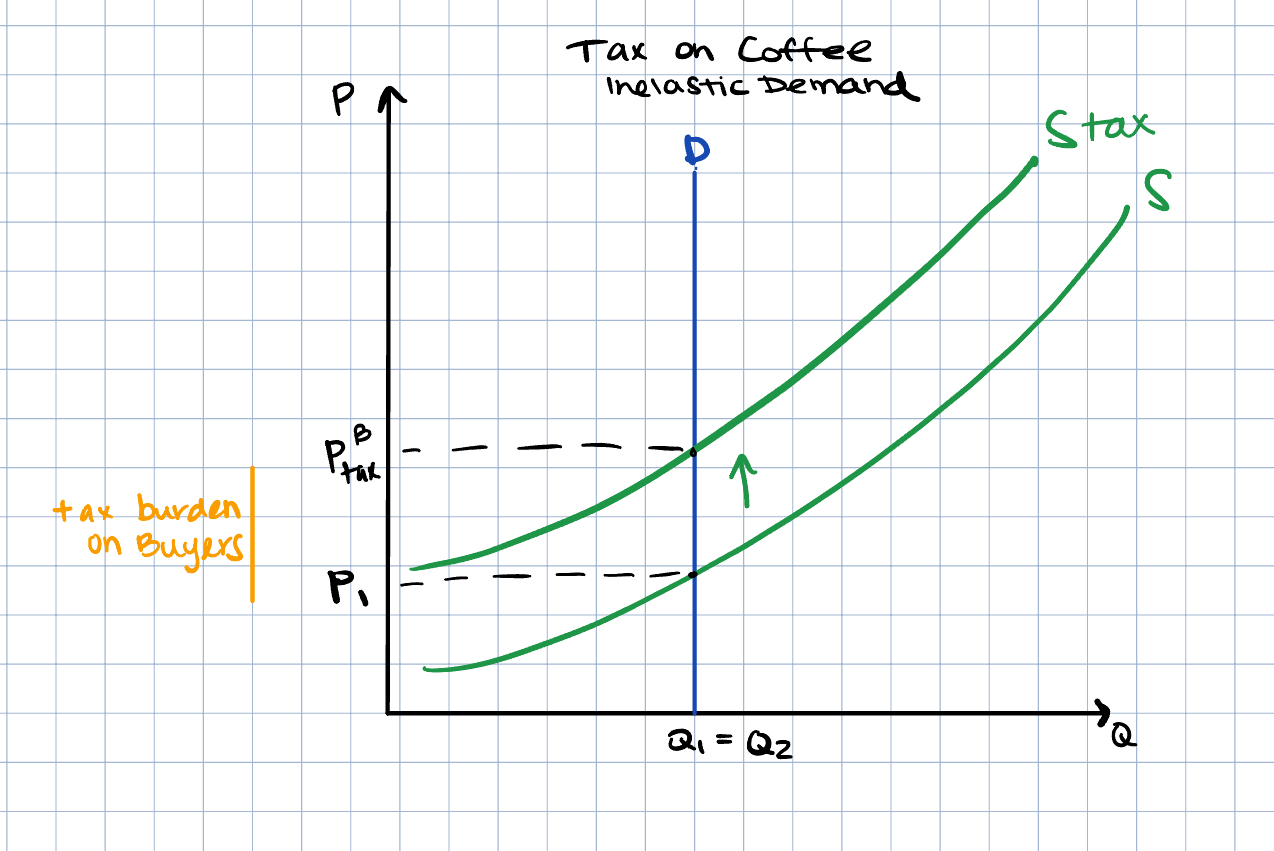
\includegraphics[width=.6\textwidth]{coffee_tax_id.png}
    \caption{Coffee tax with inelastic demand}
    \label{fig:coffee_tax_id}
\end{figure}

\begin{figure}
    \centering
    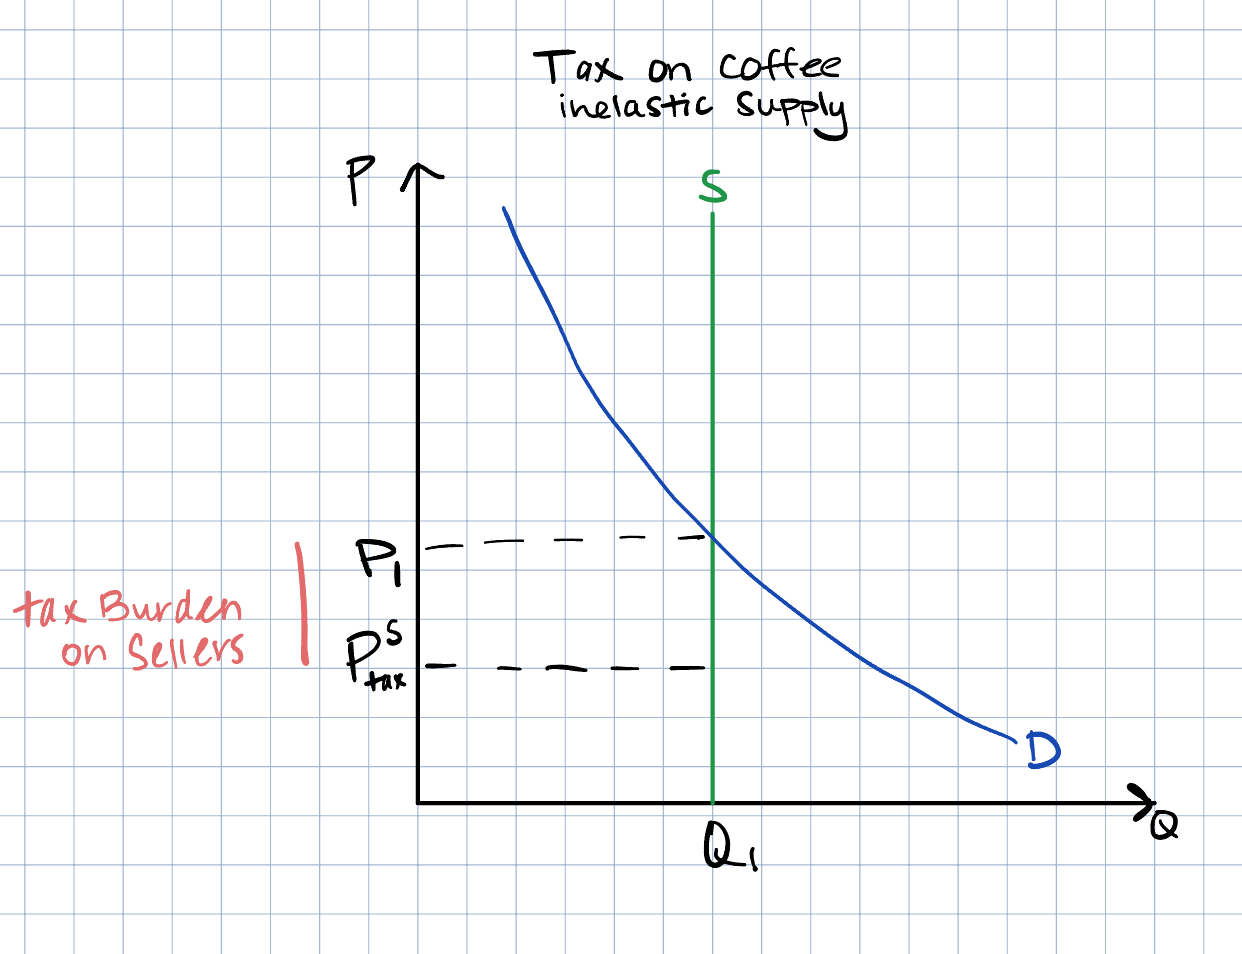
\includegraphics[width=.6\textwidth]{coffee_tax_is1.png}
    \caption{Coffee tax with inelastic supply}
    \label{fig:coffee_tax_is1}
\end{figure}

\item Repeat this exercise, but considering the tax as levied on consumers rather than producers. Does the tax burden depend on how the tax is imposed?

\textbf{Answer:}
None of the intuition is changed from before, except now it is the demand curve which shifts. Equilibrium price is now lower, because consumers have to send the \$0.5 tax to the government for each cup they buy. The quantity is lower, to the same amount as before. The tax incidence is unchanged: this is because it depends on the relative elasticities of suppliers and consumers, and not on which side of the market it is levied on.



\end{enumerate}
\end{document}
